%! TEX root = ../main.tex
\documentclass[main]{subfiles}

\begin{document}



\section{主要機能と使用技術}
本システムの主な機能とそれに対する使用技術を以下に示す.図\ref{fig:techstack}

\begin{enumerate}
\item 提案機能
\begin{enumerate}
\item メインとなるフレームワークの提案
\item その他ライブラリの提案
\item linter, formatterなどある程度共通認識が見込まれるライブラリの提案
\item ブラウザ上での実行ログの表示
\end{enumerate}
使用技術:Next.js Serverless Functions, Supabase, npm registry API, React flowなど

\item コミュニケーション促進機能
\begin{enumerate}
\item ユーザの認証・認可
\item リアルタイムチャット
\item ユーザへのロール(役割)付与
\item ユーザのオンライン・オフライン表示
\end{enumerate}
使用技術:Next.js Serverless Functions, Supabase, GraphQL, Hasura Engine, Auth0など
\end{enumerate}

\begin{figure}[h]
    \centering
    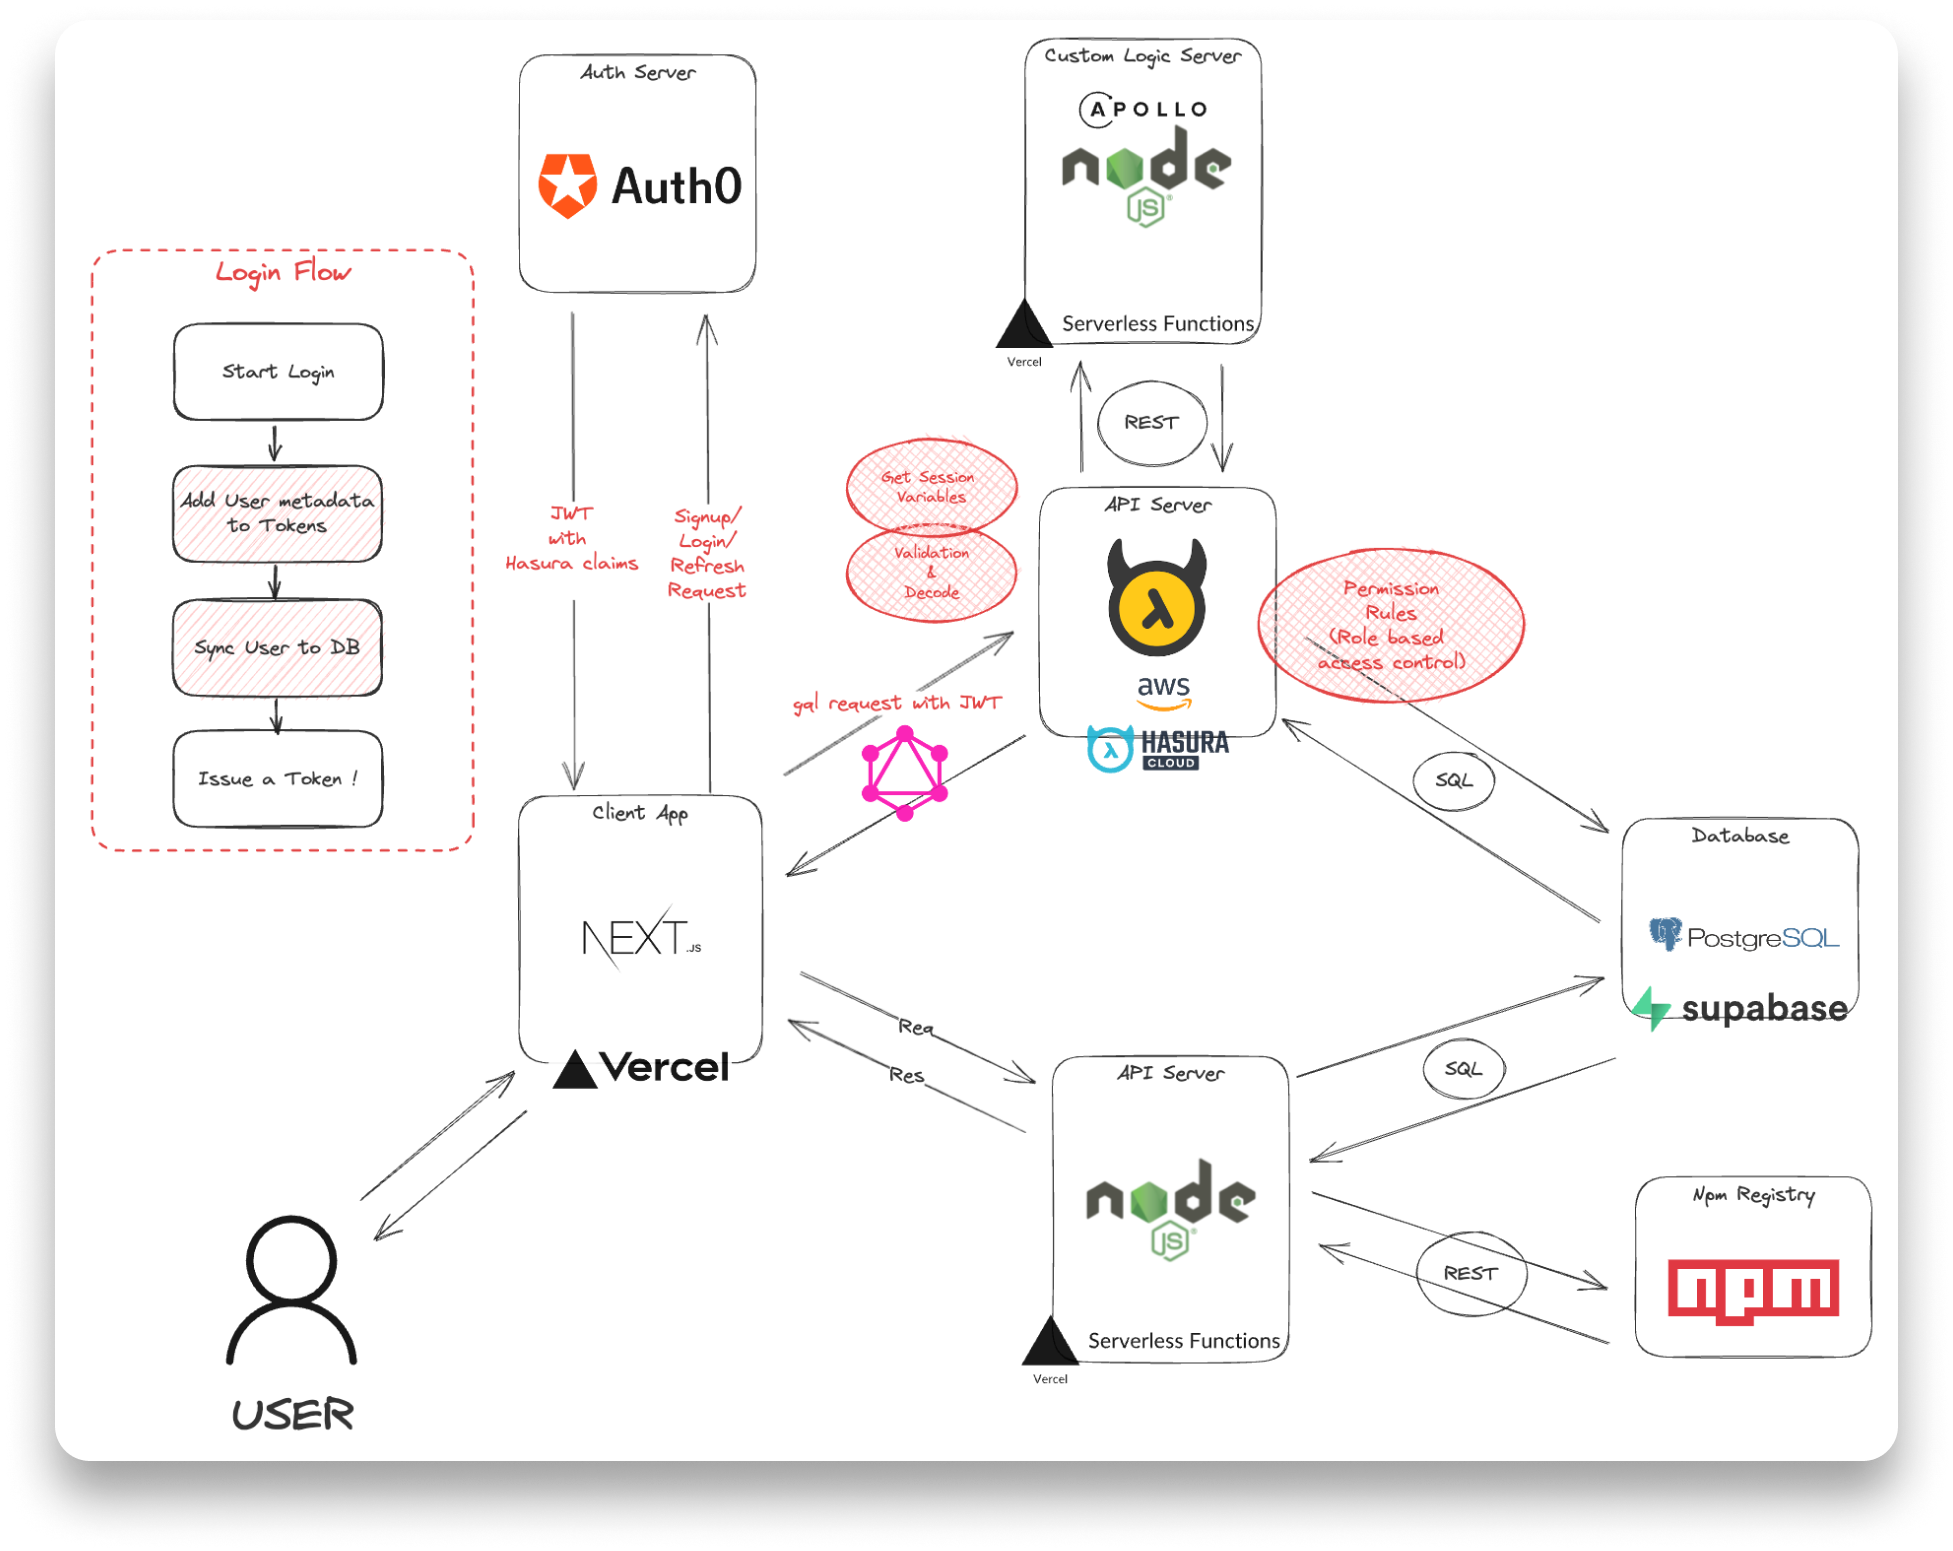
\includegraphics[keepaspectratio,width=0.9\linewidth]{../figures/techstack.png}
    \caption{技術構成図}
    \label{fig:techstack}
\end{figure}

\end{document}
